
%----------------------------------------------------------------------------------------%
% START LaTeX preamble

% define document type, font and paper size
\documentclass[11pt,a4paper]{article}

%----------------------------------------------------------------------------------------%
% IMPORT LaTeX packages

\usepackage{inputenc}
\usepackage[ngerman, english]{babel}
\usepackage{csquotes}
\usepackage{amsmath}
\usepackage{amssymb}
\usepackage{amsfonts}
\usepackage{graphicx}
\usepackage{wrapfig}
\usepackage[margin=1.25in]{geometry}

%----------------------------------------------------------------------------------------%
% IMPORT LaTeX packages to manange bibliography

% MLA, APA, or IEEE? - https://www.overleaf.com/learn/latex/Biblatex_citation_styles
\usepackage[style=apa, backend=biber]{biblatex}
\addbibresource{bibliography.bib}

%----------------------------------------------------------------------------------------%
% DEFINE header values

% define the cover page values
\title
{
    BB HOMEWORK: Planetary Boundaries Essay \\
    Analysis
}
\author
{
    Antonio Osamu Katagiri Tanaka \\
    A01212611
}
\date{\today}

%----------------------------------------------------------------------------------------%
% USER-DEFINED commands

% Keywords command
\providecommand{\keywords}[1]
{
    \\
    \\
    \small
    \textbf{\textit{Keywords:}} #1
}

%----------------------------------------------------------------------------------------%

\begin{document}

%----------------------------------------------------------------------------------------%
% CREATE the 1st page (cover page)

\maketitle

%----------------------------------------------------------------------------------------%
% DEFINE the abstract text & keywords

%\begin{abstract}
%    \emph
%    {
%        Lorem ipsum dolor sit amet, consectetur adipiscing elit, sed do eiusmod tempor incididunt ut labore et dolore magna aliqua. Ut enim ad minim veniam, quis nostrud exercitation ullamco laboris nisi ut aliquip ex ea commodo consequat. Duis aute irure dolor in reprehenderit in voluptate velit esse cillum dolore eu fugiat nulla pariatur. Excepteur sint occaecat cupidatat non proident, sunt in culpa qui officia deserunt mollit anim id est laborum.
%    }
%    \keywords{Lorem, ipsum, dolor, sit, amet}
%\end{abstract}
\clearpage

%----------------------------------------------------------------------------------------%
% CREATE a table of contents in a new page

%\tableofcontents
%\clearpage

%----------------------------------------------------------------------------------------%
% CREATE a list of figures and a list of tables in a new page

%\listoffigures
%\listoftables
%\clearpage

%----------------------------------------------------------------------------------------%
% DOCUMENT body starts here

\section{Analysis}\label{sec:intro}
Human kind is using natural resources far beyond what Earth can handle, and yet millions are living in deprivation.

In 2009 Johan Rockström along with the Resilience Alliance, came up with the concept of ``planetary boundaries". They determined that nine Earth system processes exist to keep a balance on Earth, such as: the nitrogen cycle, the freshwater cycle and climate change, see Figure \ref{Johan_planetaryBoundaries}. And, under too much pressure, any of this processes can reach a state of irreversible change, so Rockström set up a collection of boundaries between the danger zones and the area that he called the ``safe operating space for humanity". \parencite{Rockstrom2009} Rockström's approach may be environmentally safe but it could also be prone to leave millions in deprivation and extreme poverty.

\begin{figure}[!htbp]
\centering
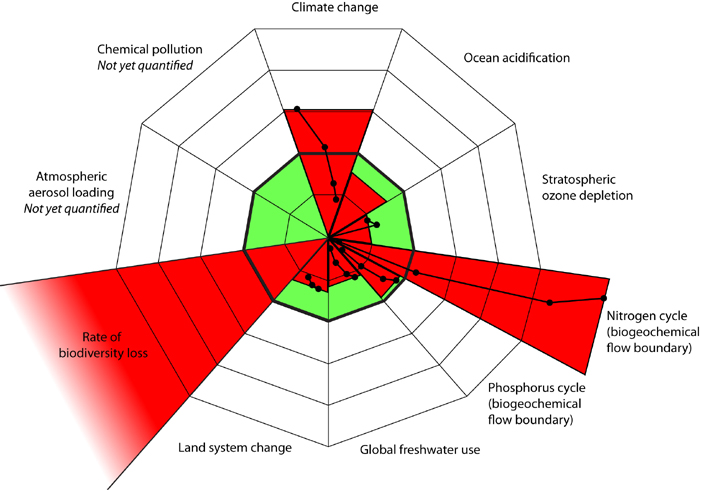
\includegraphics[width=0.70\textwidth]{img/Johan_planetaryBoundaries.png}
\caption{Planetary Boundaries \parencite{Rockstrom2009}.\label{Johan_planetaryBoundaries}}
\end{figure}

In 2012, the economist, Kate Raworth added the concept of ``social boundaries" to Rockström's diagram. Just as there is an ``environmental ceiling" (or planetary boundaries) to prevent environmantal degradation, there should also be a ``social foundation" (or social boundaries) to avert unacceptable human deprivation, as described in Figure \ref{Kate_donut}. \parencite{Raworth2012}

\begin{figure}[!htbp]
\centering
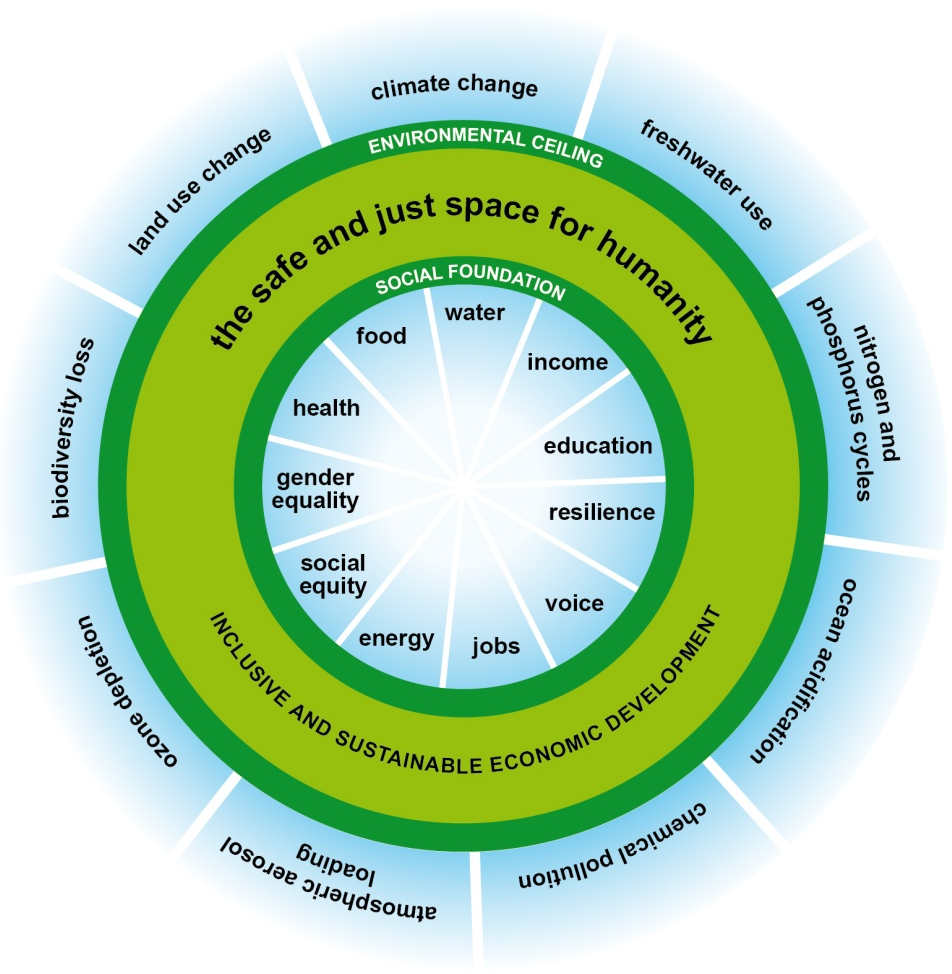
\includegraphics[width=0.70\textwidth]{img/Kate_donut.png}
\caption{A safe and just space for humanity \parencite{Raworth2012}.\label{Kate_donut}}
\end{figure}

On the other hand, Raworth introduces the concept of ``planetary health" to create a relationship between the ``social boundaries" and Rockström's ``planetary boundaries". Rockström showed that we have already overshoot our pressure on Earth, so we need to change our mindset and think about what growth looks like in terms of ``planetary health" and ``personal health". \parencite{Raworth2012}

As Raworth states, our personal health depends on food, water, shelter, health care and other things that have been recognized as human rights, however our planet health depends on a stable climate for a protective ozone layer, healthy oceans and fertile soils. So, the concept of ``planetary health" starts to connect the dots: if we want food for all, we need fertile soils and a stable climate; if we want fish in the sea, we need healthy oceans; if we want to be safe of the Sun, we need a protective ozone layer; if we want to be safe in our homes, we need a stable climate that is not prone to hurricanes. \parencite{Raworth2012}

Raworth's approach changes our idea of progress. Currently, we measure progress with economic growth. However Raworth tells us that progress is balance between using resources to meet our rights and protecting the planet's system processes.

%----------------------------------------------------------------------------------------%
% PRINT bibliography/references in a new page

\clearpage
\printbibliography

%----------------------------------------------------------------------------------------%

\end{document}

%----------------------------------------------------------------------------------------%
